% Capítulo 8: partição do quicksort com o último elemento (22) como pivô.
\documentclass[border=4pt]{standalone}
\usepackage[utf8]{inputenc}
\usepackage[T1]{fontenc}
% Estilo comum das figuras de vetores (capítulo 8).
\usepackage{tikz}
\usetikzlibrary{arrows.meta, positioning, calc, decorations.pathreplacing}
\definecolor{navy}{RGB}{23,45,80}
\definecolor{laranja}{RGB}{250,110,29}
\definecolor{cinzalogo}{RGB}{107,114,126}
\definecolor{azul}{RGB}{205,222,247}
\tikzset{
  casa/.style={draw=navy, line width=0.9pt, minimum width=8mm, minimum height=7mm,
               inner sep=0pt, font=\sffamily\small},
  pronta/.style={casa, fill=azul},
  parte/.style={casa, fill=laranja!12},
  marcada/.style={casa, fill=laranja!45, draw=laranja},
  fora/.style={casa, draw=cinzalogo!60, dashed, fill=white, text=cinzalogo!60},
  indice/.style={font=\sffamily\scriptsize, text=cinzalogo},
  explica/.style={font=\sffamily\small, text=navy, anchor=east},
  legenda/.style={font=\sffamily\scriptsize, text=cinzalogo},
  rotulo/.style={font=\sffamily\small\bfseries, text=navy},
  seta/.style={-{Stealth[length=2.2mm]}, navy, line width=0.9pt},
  chave/.style={decorate, decoration={brace, amplitude=4pt, mirror}, navy, line width=0.8pt},
}
% \vetor{nome}{x}{y}{valor/estilo, valor/estilo, ...}: casas lado a lado, chamadas nome0, nome1...
\newcommand{\vetor}[4]{%
  \foreach \valor/\estilo [count=\i from 0] in {#4} {
    \node[\estilo] (#1\i) at ($(#2, #3) + (\i*0.8, 0)$) {\valor};
  }
}

\begin{document}
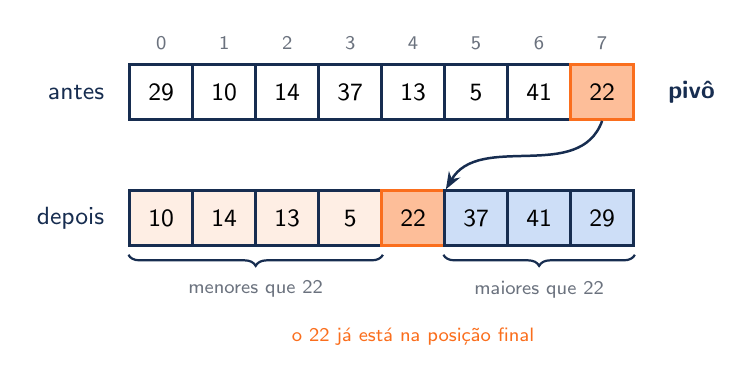
\begin{tikzpicture}
  \node[explica] at (-0.6, 0) {antes};
  \vetor{a}{0}{0}{29/casa, 10/casa, 14/casa, 37/casa, 13/casa, 5/casa, 41/casa, 22/marcada}
  \foreach \i in {0,...,7} { \node[indice, above=0.5mm of a\i] {\i}; }
  \node[rotulo, right=3mm of a7] {pivô};
  \node[explica] at (-0.6, -1.6) {depois};
  \vetor{b}{0}{-1.6}{10/parte, 14/parte, 13/parte, 5/parte, 22/marcada, 37/pronta, 41/pronta, 29/pronta}
  \draw[seta] (a7.south) to[out=-110, in=60] (b4.north east);
  \draw[chave] ([yshift=-1mm]b0.south west) -- node[legenda, below=2mm] {menores que 22} ([yshift=-1mm]b3.south east);
  \draw[chave] ([yshift=-1mm]b5.south west) -- node[legenda, below=2mm] {maiores que 22} ([yshift=-1mm]b7.south east);
  \node[legenda, below=9mm of b4, text=laranja] {o 22 já está na posição final};
\end{tikzpicture}
\end{document}
